\documentclass{standalone}

\graphicspath{{img/Chap1}}
\begin{document}

\chapter{Preliminary Knowledge}\label{CAP:theory}

The aims of this work of thesis was to prepare head MR images for a segmentation using a U-Net and then to refine the outcomes cleaning the misclassified ones.
In order to do that different techniques was used and is necessary to briefly define, show and explain the approaches used.
In this chapter, medical images are briefly introduced, then the main segmentation techniques used are illustrated; finally, the metrics useful for evaluating the results obtained are treated.

% Non ho assolutamente un'idea di cosa scrivere o come chiamare il capitolo. L'idea di base è che questi sono i principi teorici che poi ho usato nell'implementazione ma non ho davvero una cazzo di idea di come minchia scriverlo! <3 


\section{Medical Images}
An image is a collection of measurements in two-dimensional (2-D) or three-dimensional (3-D) space \cite{ART:Pham}.
A medical image is a discrete representation of the internal structure or function of an anatomic region in form of a tensor of picture elements called pixels/voxels. A pixel is a discrete numeric representation of intensity or gray-level\cite{mastersthesis:Filitto}. The representation results from a process that maps every numerical value in a position in space and the number of picture elements involved express the level of detail with which the subject will be depicted \cite{mastersthesis:Biondi}.
The physical meaning of the numerical value of a pixel changes according to the imaging modality, the acquisition protocol, the reconstruction and eventually the post-processing.
Nevertheless there are 4 concepts in common for every medical image: \texttt{pixel depth, photometric interpretation, metadata} and \texttt{pixel data} \cite{ART:Larobina}.
In the following lines these characteristics will be rapidly described.

\paragraph{Pixel Depth}
Pixel depth is the number of bits used to encode the information stored in each pixel. A higher number of bits per pixel permits to store a greater information but requires a greater usage of memory \cite{ART:Larobina}.
We can exemplify the concept just expressed considering a square image with a side of $256$ pixel of depth $2 \ bytes = 16 \ bit$ ($1 \ byte = 8 \ bits$). In this case each pixel can express $2^{16} = 65,536$ levels which are usually arranged as integers in range $[0; 65,535]$. It is also possible store the values in the interval $[ -32,768; 32,767] $ using 15 bits to store the level and a bit to represents the sign. In this example the image will occupy $256 \times 256 \times 2 = 131,072 \ bytes$.

It is to mention also the possibility for a pixel to store a real number. For this case the Institute of Electrical and Electronics Engineers created a standard (IEEE-754) in which defines two basic formats for the binary encoding of a floating point number: \textit{single precision} with $32 \ bit$ depth and \textit{double precision} with $64 \ bit$ depth.

\paragraph{Photometric Interpetation}
The photometric interpretation specifies how the pixel data should be interpreted for the correct image display as a monochrome or color image. To clarify that sentence it is useful to introduce the concept of \textit{number of channels}, also known as \textit{sample per pixel}. Monochrome images have only 1 sample per pixel and all the bits in the pixel depth is used to represents the gray level ~\cite{ART:Larobina}.
Typically x-ray computed tomography (CT) and magnetic resonance (MR) images are monchrome, and so, in that elaborate, we will mainly consider those kind of images.
Furthermore nuclear medicine images, such as positron emission tomography (PET) and single photon emission tomography (SPECT) the data are usually visualized with a color map, that map is however predefined and the colors are not information stored in the pixels. In that case the number of channels is 1 and that images are usually referred to be in \textit{pseudo-color}.
To encode color information into pixels is necessary to have more than one number of channels. It is common to have RGB (Red, Green and Blue) images, which are composed of 3 channels. In this case the pixel depth can be obtained multiplying the number of bits per channels (usually 8 bits \cite{Graphic_encyclopedia}) for the number of channels \cite{ART:Larobina}.
An example of colored images in medical usage are the Doppler ultrasound in which the color is used to encode blood flow direction and velocity. \cite{mastersthesis:Biondi}.


\paragraph{Metadata}
Metadata are informations that describe the image. It is usually stored at the beginning of the file as a header and contains at least the image matrix dimensions, the spatial resolution, the pixel depth, and the photometric interpretation \cite{ART:Larobina}.
Using the metadata, advanced medical image visualization software are able to correctly read, display and elaborate medical images if the format is supported.
In medical images metadata acquires an also greater importance due to the nature of the images itself. It is possible to store information about how the image was produced and even informations on the patient~\cite{mastersthesis:Biondi}.

\paragraph{Pixel data}
Pixel data represents the numerical value stored in the pixel. According to the data type, pixel data are stored as integers or floating point numbers.
Although is not common, it is also possible to store complex numbers in pixels. An example is pixel data from MRI before the reconstruction that provides informations about both the phase and the intensity (The so called \textit{k-space})~\cite{ART:Larobina}.

\subsection{Medical Image Format}
Image file formats provide a standard way to store the information describing how the image data are organized inside the image file and how the pixel should be interpreted by software for the correct loading and visualization.
First of all, it is necessary to distinguish between two main categories of formats: The first is intended to standardize the images generated by diagnostic modalities and the seconds has the purpose of facilitate and strengthen post-processing analysis \cite{ART:Larobina}. The example here discussed are \texttt{DICOM} for the first category, that is the original file format of the datas analyzed in that paper, and \texttt{Nifti} for the second category, which is the format mainly used during during this thesis work.

\paragraph{DICOM}
The Digital Imaging and COmmunications in Medicine (which acronyms is \texttt{DICOM}) standard was established by the American College of Radiology and the National Electric Manufacturers Association in 1993 and was introduced in imaging departments a the end of the '90s. Now it is the backbone of every medical imaging department, also because it is not only a file format but also a network communication protocol. The value of \texttt{DICOM} is that the pixel data and the description of the medical can't be separated, accentuating the concept that an image is quite meaningless without its metadata and so they are merged in a unique file. The \texttt{DICOM} header contains a full description of the entire procedure used to acquire the image, including patient information such as name, gender, age, weight, and height~\cite{ART:Larobina}.
It has 2 main limitations: As a matter of fact pixel that can only store integer values (altough floating point data can be stored in the metadata), and also it is born for only 2D images, so a 3D volume is described by a series of files containing the single slices~\cite{mastersthesis:Biondi}.


\paragraph{Nifti}
The \texttt{Nifti} format was originally created at the beginning of 2000s by a committee based at the United States' National Institutes of Health (known as NIH)~\cite{ART:Larobina}.
It's strength is due to the header that can store information about image orientation image centre and origin, and that can, for example, resolve ambiguity between left and right in brain hemisphere MRI.
It is supported by many software of image viewing and can store 3D images. For those reasons it is the format used in this work.



\section{Magnetic Resonance Imaging (MRI)}
Magnetic Resonance Imaging is an imaging technique base on the physics phenomenon of Nuclear Magnetics Resonance (NMR), a process that involves the magnetic moments of the atoms that, immersed in a constant magnetic field, align themselves with the external magnetic field, giving rise to a small paramagnetic polarization contrasted only by the thermal agitation. 
The constant magnetic field also give rise to a phenomenon called \textit{Larmor precession}, in which the nuclei's magnetic moment precess  around the external magnetic field direction with a particular frequency, called \textit{Larmor frequency}, dependent on the external field.
Applying an oscillating magnetic field, perpendicular to the constant magnetic field (z axis), at the Larmor frequency puts in resonance the nuclei, which magnetic moment's latitude will change accordingly to the magnetic pulse received. Inserting in the apparatus a coil with axis perpendicular to the plane where lie the magnetic fields, it is possible to register an oscillating induced voltage \cite{ART:Bloch}.

The nuclei, immersed in the constant magnetic field, will tend  to come back to their original orientation once the oscillating magnetic field is turned off.
NMR informations, and in particular the ones needed for the recording of an MRI images, comes just from the relaxation time of the magnetic polarization, that is the time needed for the vector to return parallel to the constant field. It is necessary to underline that magnetic polarization is a vector and so it can be splitted in two components, one longitudinal (z axis) and one transversal (xy plane). The relaxation is so defined as the time to made the transversal component go back to $0$ and the longitudinal component return to the initial value. Those two processes has different individual relaxation times: $T_1$ for the longitudinal component and $T_2$ for the transversal component.
The processes of realignment in longitudinal and transversal directions have different natures.
The longitudinal relaxation for a nucleus is due to the interaction of the spin with the lattice and so the T1 time is also called \textit{spin-lattice relaxation time}.
The transversal relaxation otherwise is due to the interaction between the nucleus' spin with other spins, then the T2 time is also called \texit{spin-spin relaxation time}.
It is also to be noticed that the T1 time is longer than T2.
This process of relaxation produce a signal called Free Induction Decay (FID) that is the signal registered.

\subsection{Pulse Sequences Images}
In MRI the constant magnetic field is usually not uniform, but has a gradient. The presence of a not uniform field lead to nuclei with different Larmor frequency depending on their displacement in the space. Adjusting the frequency of the pulsing field is possible to select only a small slice of space in which nuclei will have that determined resonance frequency.

It is possible to obtain different contrast between tissues applying particular sequences of impulses for the oscillating magnetic field that permits to maximize or minimize the effect of some particular physics phenomena of the FID. It is, for example, the case in which the FID from T1 relaxation time or the T2 relaxation time are maximized, as briefly explained below. Another example of phenomena which FID can be maximized is the diffusion, but they wouldn't be treated because are not relevant for this work of thesis. In the next lines will be briefly discussed the main images obtained by the different sequences and the most used during the work.

\paragraph{T1-Weighted}
T1 Weighted image (also referred as \textit{spin-lattice}) is one of the more frequently recorded image modality in MRI and demonstrates differences in the T1 relaxation times of tissues. For example fat's longitudinal magnetization realigns rapidly  with $B_0$, and it therefore appears bright. On the contrary water has a slower relaxation time in the longitudinal axis and therefore has a lower signal appearing dark \cite{T1}.

\paragraph{T2-Weighted}
T2 Weighted image (known also as \textit{spin-spin}) is also one of the basic pulse sequences on MRI and highlights differences on the $T_2$ relaxation time of tissues \cite{T2}.
In this kind of images the water appears bright and conversely fat appears darker than the T1-w images.
T2-weighted images are often most helpful for assessing areas of pathology because diseased or injured tissue contains a higher water content than is normal, resulting in signal hyperintensity \cite{ART:Finkelstein}.

\paragraph{FLAIR}
FLuid Attenuated Inversion Recovery (FLAIR) is a special sequence that removes signal from the cerebrospinal fluid in the resulting images. Brain tissue on FLAIR images appears similar to T2W images with grey matter brighter than white matter, but cerebrospinal fluid (CSF) is dark instead of bright.
It is very useful in evaluating cerebral infarts and multiple sclerosis lesions because they will appear hyperintense in this kind of images \cite{FLAIR}.


\begin{figure}[h!]
		\centering
        \begin{subfigure}[b]{0.325\textwidth}
             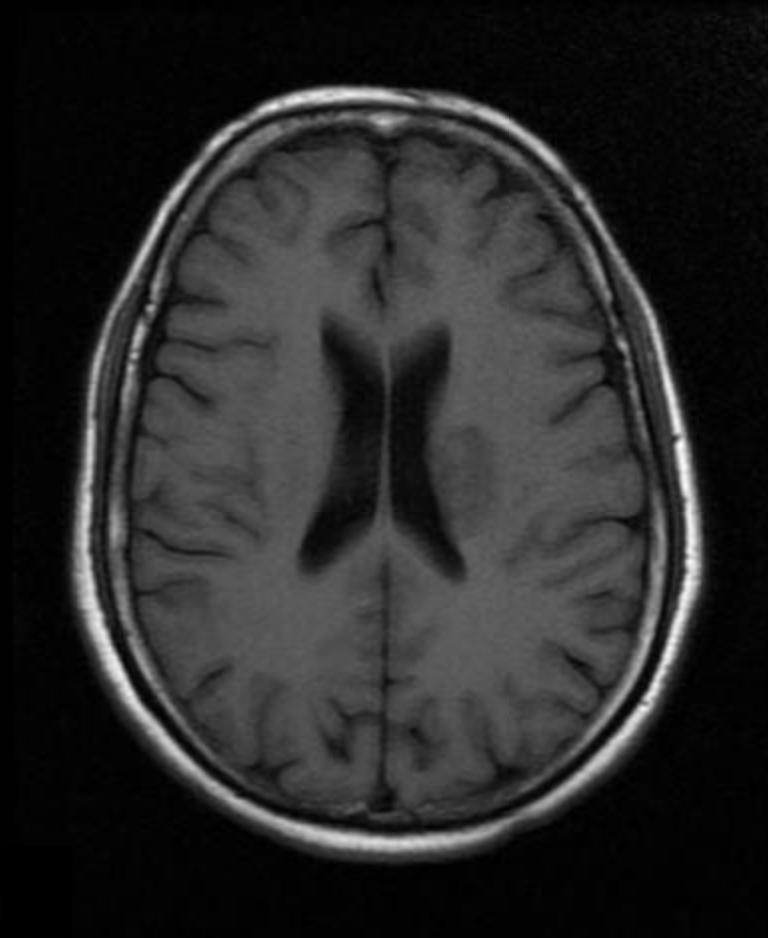
\includegraphics[scale=0.365]{img/Chap1/T1_example.png}
             \caption{T1-W image}
             \label{fig:T1_example}
        \end{subfigure}
        \hfill
        \begin{subfigure}[b]{0.325\textwidth}
             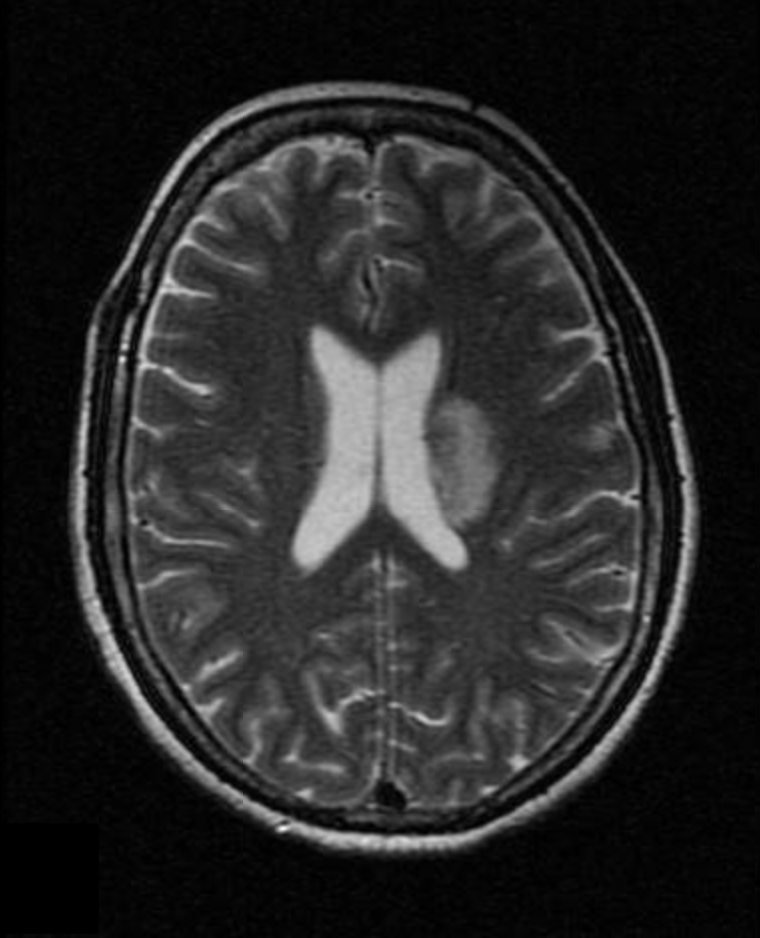
\includegraphics[scale=0.365]{img/Chap1/T2_example.png}
             \caption{T2-W image}
             \label{fig:T2_example}
        \end{subfigure}
        \hfill
        \begin{subfigure}[b]{0.325\textwidth}
             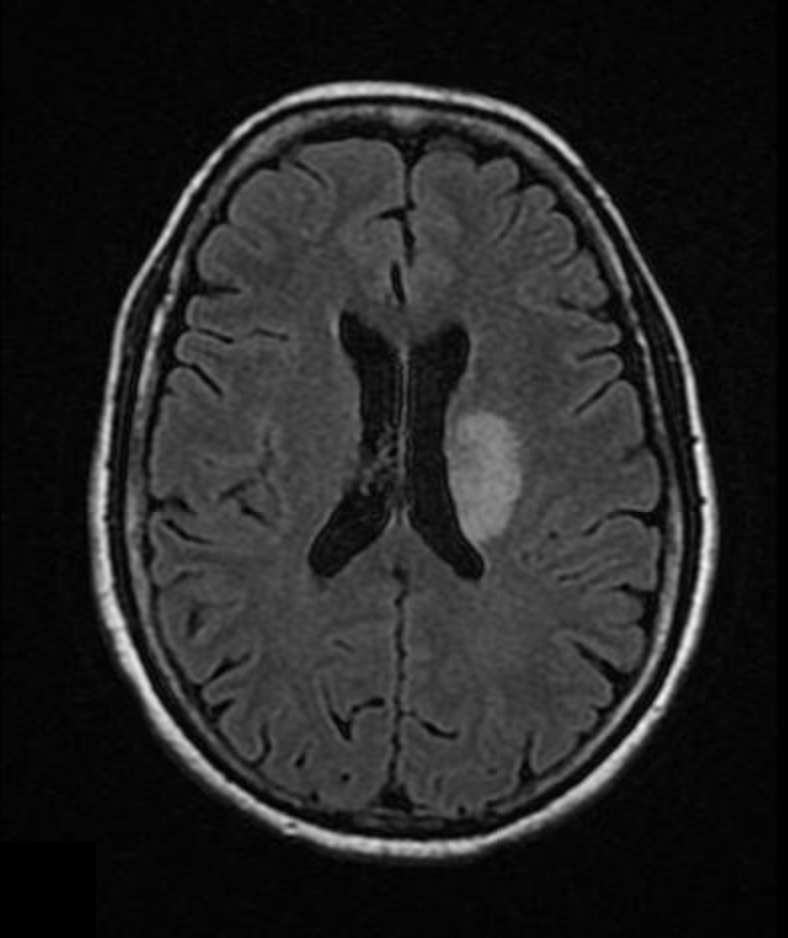
\includegraphics[scale=0.365]{img/Chap1/FLAIR_example.png}
             \caption{FLAIR Image}
             \label{fig:FLAIR_example}
        \end{subfigure}
		\caption{Comparison between 3 images obtained with different pulse sequences of the same brain \cite{IMG:PulseSequences}. It is possible to observe how the cerebrospinal fluid (CSF), the white matter (WM) and grey matter (GM) appear in the different images. The lesion here observable therefore appears hypointense in the T1W image and hyperintense in the T2W and FLAIR images.}
		\label{fig:Modality_comparison}
	\end{figure} 

\subsection{Image Acquisition Type}
As explained in the previous section, in MRI the resonance is possible to encode spatial information by using a magnetic gradient, due to the dependency of the Larmor frequency on the intensity of the local magnetic field.
Traditionally this effect was used to select only a small slice of tissue and the image recorded was in two dimensions.
The MRI volume was in this case recorded as a set of planar images.
In more recent years another technique has been developed that permits to record a volume in its integrity, obtaining images with truly cubic voxels and with a higher resolution \cite{ART:Martì}.

\subsubsection{2D Imaging}
In two dimensional imaging a constant field with a gradient is applied on the z axis and a selective radiofrequency pulse is applied on the xy plane. In this way only the nucleis on a small slice will be excited and that permits to select only a set of voxels in an xy plane.
The spatial informations about the remaining two dimensions (x and y) are provided by an encoding of frequency and phase.

It is possible to select thinner slices increasing the gradient on the z axis but there is a limitation to the thickness that can be choose. Usually is difficult to select slices of a thickness lower than $3\ mm$. This is due to the Signal-to-Noise ratio (SNR) because smaller voxels will produce a lower signal. 
This will cause to have voxels that represent volumes with different tissues in it, this is the so called \textit{partial volume effect}.
Also the slices are usually separated by a gap of non included tissue to prevent overlapping between successive slices.

The result of this acquisition technique is then a set of 2D images with a low resolution on the z axis \cite{ART:Martì}.

\subsubsection{3D Imaging}
In 3D imaging the constant field on the z axis has not a slice selecting gradient and the entire sample volume is excited simultaneously. The spatial information on the z axis is provided by another phase encoding.
3D images can be seen as a rectangular box that delimits the anatomic region in all dimensions subdivided in smaller contiguous voxels. In 3D scans voxels are usually isotropic, which means that have the same dimensions in all the three axis.
The images acquired with a 3D technique have usually a greater spatial resolution and having smaller voxels permits to reduce the partial volume effect.



\section{Registration}
Image registration is an image processing technique used to align and overlay two or more different images or volumes.
The need for a registration appear whenever it is necessary to compare two images containing different informations about the same subject \cite{ART:Junchi} or also when a study on many patient is done and there is the need to have all the volumes in the same space. An example in medical field can be the case in which it necessary to compare two images of the same patient taken with different impulse modalities (i.e. T1-W and FLAIR). In this case, the examined anathomical structure is the same, however the two images are not necessary overlapping. That because may happen that a patient change his position during the exam.   
An other use case may be in case of multi-patients studies, where there is the necessity to compare the different images to an atlas. 

Image registration process involves two images: a moving image ($I_m(x)$) which is moved and deformed, and a fixed image ($I_f(x)$), which is the reference one. The registration process allows to find the transformation ( $T(x)$) which allows the moving image overlay the reference one. The best transform is estimated by minimizing a certain \emph{cost function}. This function has to be chosen according to the image type and registration purposes \cite{ART:Elastix}, since different types of cost functions can lead to very different results in the registration process.
An example of of this cost function can be the \emph{mean squared error} between the pixel intensities of the fixed and moving image. This kind of function can have good results registering two images acquired with the same modality but would not work properly in registering images acquired with different modalities (e.g. a T1W scan and a FLAIR scan), because the same tissue have different pixel values in the two images.
In this cases other metrics are more effective, for example the \emph{mutual information}.

There is the possibility to distinguish between two kinds of process that lay under the name of registration. In the first meaning the word is used to indicate the process of finding a transformation that can relate the position of features in one image with the position of the corresponding feature in another image. The second meaning both relates the position of corresponding features and enables us to compare the intensity at those corresponding positions. In this second meaning the concepts of \textit{resampling} and \textit{interpolation} are incorporated \cite{ART:Hill}.  
Resampling is the process in which the orientation, resolution or field of view of an image is changed \cite{Slicer_Resampling}. In image registration this could be necessary because the sampling grid of the original moving image is modified by the applied transformation.
Due to the changing of sampling of the moving image it appear the problem of finding the pixel intensities for the new pixels in the transformed grid. This can be done estimating the new values starting from the original ones and taking into account the transformation applied to the image. This process is called interpolation. 

Another aspect to take in account is the type of transformation that can be applied to the moving image. They can be subdivided by the \textit{degrees of freedom (dof)} of the transformation:
\begin{itemize}
    \item \textbf{Rigid} transformation allows 6 dof. In this kind of transformation the image is treated as a rigid body which undergoes to rotation (3 dof) and translation (3 dof) along the axis. In medical application is usually applied when the subject of the image is rigid (e.g. a bone) or when the two images are acquired with the same modality but with a time lapse between the two acquisitions;
    
    \item \textbf{Affine} transformations allows 9 or 12 dof. This kind of transformations incorporate also scale (3 dof) and skews (3 dof) besides rotation and translations.
    Even if for the nature of the biological organs this approach don't increase greatly the applicability of image registration, because usually organs don't only stretch or shear, this kind of transformation is useful for overcoming scanner induced errors \cite{ART:Hill};
    
    \item \textbf{Non-affine} transformations have an indefinite number of dof and allows also the deformation of the moving image. 
    There are many different non affine transformations which uses different approaches. For example the non-rigid component of the transformation can be determined using a linear combination of polynomial terms, basis functions, or B-spline surfaces \cite{ART:Hill}.
    An interesting example of non-affine approach is the deformation grid, in which a grid is overimposed on the moving image and then stretched and deformed to match the fixed image.
\end{itemize}






\section{Segmentation}
Image segmentation is defined as the partitioning of an image into non-overlapping, constituent regions that are homogeneous with respect to some characteristic such as intensity or texture \cite{ART:Pham}. 
The segmentation of an image have a great relevance for medical purposes because it can help extracting features that provides informations about organ volumes or lesions identification \cite{mastersthesis:Biondi}.
Usually it can be performed identifying a surface for each tissue class (\textit{boundary identification}) or by the classification of each pixel in the volume (\textit{volume identification}) \cite{ART:Withey}.
The classification of image segmentation techniques is challenging or even impossible because of the different criteria that can be used. One classification criteria can be defined by the segmentation outcome:  \emph{hard-segmentation} that returns a net assignment of a pixel to a determined class, or \emph{soft-segmentation}, where the output is a map of probabilities to belong to each class. It is always possible to transform a soft-segmentation to a hard-segmentation by applying a threshold to the probability value.

Another possible classification for the segmentation process depends on the degree of human interaction required to achieve the segmentation. Using this criterion we can distinguish between \emph{manual}, \emph{semi-automatic} or \emph{automatic} segmentation.

\paragraph{Manual segmentation}
technique requires a trained and high specialised operator that has to visually recognise and identify the searched region. The operator usually visualize the images using specialized softwares and manually annotates them. Right now it is still the most reliable and precise technique but it ha the disadvantages to be highly time consuming and operator-dependent \cite{mastersthesis:Filitto}.

\paragraph{Semi-automatic segmentation}
techniques requires a limited interaction by an human operator to set the parameters for the image segmentation.
Those techniques includes operation like clustering and thresholding in cases where the parameters are not predetermined but has to be manually set for each volume.
Another highly used semi-automatic set of applications are the ones in which the images are firstly roughly segmented automatically and then manually corrected by an operator.
While this approach permits to save time it keeps being operator-dependant.

\paragraph{Automatic segmentation}
Thanks to the improvement of computer power it began possible a fully automatic segmentation, which means that no human interaction is needed. Often done with the help of Artificial Intelligence (AI) as in case of Neural Networks \cite{ART:Biondini}.
This technique is faster and totally operator-independent, but it is hard to implement\cite{mastersthesis:Filitto} and is still in a development state.

\subsection{Principal Segmentation Methods}

During the years in literature are appeared several techniques on medical image segmentation. When approaching a segmentation more than one of those techniques can be combined into pipelines to obtain the best results \cite{ART:Pham}.
In the following lines will be described the ones used in this work.

\subsubsection{Thresholding}
Thresholding approach segment a scalar image by creating a binary partitioning of the image intensities \cite{ART:Pham}.
In thresholding the main goal is to find the threshold that divides the histogram of the intensity occurrences of the image in two classes, one with intensities higher and one with intensities lower than the threshold, that are physically significant. An example of thresholding segmentation can be seen in Figure \ref{fig:Threshold}.

It is common that more than two classes has to be find and in this case the process is called \textit{multithresholding} \cite{ART:Pham}.
The simple application of a thresholding (or mutithresholding) approach is often not sufficient to obtain a proper segmentation due to the presence of noise or intensity nonuniformity, often found in medical images. Despite that thresholding continue to be used, due to its semplicity, when the problem permits it or as a step in a more complex approach\cite{ART:Withey}.

\begin{figure}[h!]
		\centering
        \begin{subfigure}[b]{0.325\textwidth}
             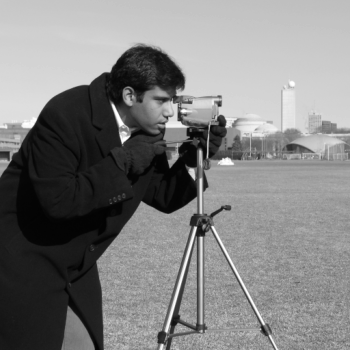
\includegraphics[scale=0.38]{img/Chap1/THR_original.png}
             \caption{Original Image}
        \end{subfigure}
        \hfill
        \begin{subfigure}[b]{0.325\textwidth}
             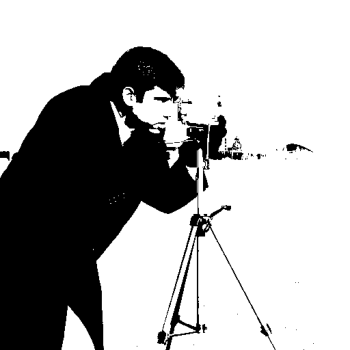
\includegraphics[scale=0.38]{img/Chap1/THR_thresholded.png}
             \caption{Thresholded Image}
        \end{subfigure}
        \hfill
        \begin{subfigure}[b]{0.325\textwidth}
             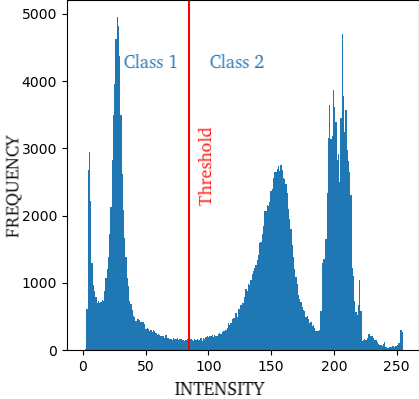
\includegraphics[scale=0.35]{img/Chap1/THR-histogram.png}
             \caption{Image Histogram}
        \end{subfigure}
		\caption{Example of thresholding application to a common image \cite{IMG:Threshold}. In this case the aim of the segmentation was to recognise the subject (class 1) from the background (class 2). In the histogram image (c) it is possible to see the two classes and the threshold division. 
		        }
		\label{fig:Threshold}
	\end{figure}

\subsubsection{Statistical Pattern Recognition}
The statistical pattern recognition field groups many different techniques of segmentation.
Even if giving a proper definition is not easy, it is possible to summarize the concept of saying that it consists in the automatic discovery of regularities in data through the use of computer algorithms and with the use of these regularities to take actions such as classifying the data into different categories \cite{Bishop}.

In order to do that classification it is necessary to evaluate a set of \textit{features} for each pixel.
A feature is an individual measurable property or characteristic of the pixel itself \cite{Bishop}. This changes from the original variables (the image) to some new variables (the feature) is aimed to make the pattern recognition problem easier to solve \cite{Bishop} as those features forms a set of patterns and the classification of that patterns permits the classification for each pixel \cite{ART:Withey}.
For example the more common visual features include color (or grey level in 1-channel images), shape or texture \cite{ART:Zheng}.

The pattern recognition techniques are usually classified in \textit{supervised} or \textit{unsupervised} depending on their need for a set of example target labels in the training set or not.
In this section some of the main used pattern recognition techniques will be briefly discussed, such as \emph{classifiers} as a supervised approach and \emph{clustering} for unsupervised.

\paragraph{Classifiers}
need for an already labeled set in the training stage and so they are considered as a supervised approach. The training data is usually manually segmented to let the classifier learn how the features can lead a pixel to belong to a class or another. Once trained the statistical classifier can assign to every pixel a probability of belonging to each class, based on the extracted features.
The main disadvantage of this approach is the necessity for human work to collect the training set. Those training data must be sufficiently large to offer to the classifier enough variability in the set, otherwise the classifier risks to over specialize only on the training data \cite{ART:Pham, ART:Withey, mastersthesis:Biondi}.



\paragraph{Clustering}
doesn't require labelled training examples since it is an unsupervised approach. This approaches usually require an initial choice of parameters from which they are particularly dependent \cite{ART:Pham, mastersthesis:Biondi}.
For brain segmentation usually the number of clusters is previously known and so it is frequent that algorithms that needs this parameter as input are used. Three from the most used algorithms of that kind will be briefly explained in the next lines as examples:
\begin{itemize}
	
		\item \textbf{k-means clustering:} it permits to partition $n$ ($X(x_1,x_2,...,x_n)$) pixels in $k$ clusters and minimize the distance function 
		($\sum_{i=1}^{k} \sum_{j=1}^{n} ( x_{ij}-C_{i} )^2 $) where $C_i$ represents the i-th cluster center.
		The k-means algorithm than follows this steps \cite{ART:Qiao}:
		\begin{enumerate}
		    \item Initialize cluster centroids with random samples;
		    \item Assign each observation ($x_i$) to the nearest cluster center;
		    \item Recalculate and update each cluster center ($C_i$);
		    \item Repeat steps 2 and 3 until $C_i$ does not change.
		\end{enumerate} 
		
		\item \textbf{Fuzzy C-means: } this algorithm is a generalization of the k-means clustering that permits \textit{soft-segmentation}. Intuitively, the degree to which a pixel belongs to a cluster is inversely proportional to the distance from the pixel to the center of that cluster. In this algorithm the function to minimize is always a distance between each pixel and the cluster's centroids, but it is weighted over the probability of belonging to the determined class \cite{ART:Lauric};
		
		\item \textbf{Expectation Maximization:} In this approach the pixel intensities of each tissue are supposed to follow a Gaussian distribution. The distribution of the pixel intensities of the whole image is supposed to follow a Gaussian Mixture distribution. The Gaussian Mixture can then be defined as 
  \begin{equation}
      p(x) = \sum_{k=1}^K \pi_k N(x|\mu_k, \Sigma_k)
  \end{equation} \label{EQ:GaussianMixture}
        where $\{1, 2, ..., K\}$ is the set of mixture components and, for the $k$-th mixture component, $\pi_k$ is the mixture weight and $ N(x|\mu_k, \Sigma_k)$ is a d-variate Gaussian density, $\mu_k$ is the mean vector and is the covariance matrix.

        The Expectation Maximization algorithm follows then this steps \cite{ART:Qiao}:
        \begin{enumerate}
            \item Initial parameters are somehow initialized (randomly, by k-means or manually given) and then the log likelihood is computed;
            \item The posterior probability is computed using the current parameters (\texttt{Expectation} step);
            \item The parameters are recalculated from the current posterior probability (\texttt{Maximization} step);
            \item The log likelihood is recomputed;
            \item Repeat step 2, 3, and 4 until a predetermined convergence criterion is satisfied.
        \end{enumerate} 
        
        
        
  \end{itemize}


\subsubsection{Neural Networks}
Artificial Neural Networks(ANN) are a computational architecture derived from neural physiological models \cite{mastersthesis:Biondi}.  In this network each node can perform elementary computations, adapting the weight assigned to the connections between nodes gives to the network a property similar to the biological capacity of learning \cite{ART:Pham}.
This brings out the necessity for a training stage, in which the network can compare a set of features for a pixel with the classification outcome. After this step it is possible to give some new data to the ANN and it will classify them according to the data received during the training step \cite{ART:Withey}.

There are many different architectures for Neural Networks but one of the more used in image segmentation is \textbf{Convolutional Neural Network (CNN)} \cite{mastersthesis:Biondi}.
CNNs are part of the class of Deep Learning Networks. It's typical structure can be divided in \textit{input layer}, which represents the set of data, then quantity of \textit{hidden layers} and finally the \textit{output layer} which provides the results of the segmentation \cite{mastersthesis:Filitto}.
In this kind of architecture for image segmentation, the hidden layers usually belongs to three categories:
\begin{itemize}
    \item \textit{Convolutional layers} is made of several convolutional kernels that iteratively convolves local regions of the inputs to generate feature maps. The output of a convolutional layer is a tensor of fetaures. Usually this layer is followed by the application of an activaton function;
    
    \item \textit{Pooling layers} which performs subsampling at their input data. For example they can take inputs from a $2 \times 2$ unit region in the corresponding feature map (from the convolutional layer) and would compute the average of those inputs. This stage permits to achieve invariance respect small shifts of the image in the corresponding regions of the input space \cite{Bishop}. Pooling layers are usually placed in between two convolutional layers;
    
    \item \textit{Fully connected layers} that is a layer in which every possible connection between the input and the output layers can be found. It can be usually find after several convolutional and pooling layers in order to perform high-level reasoning
\end{itemize} 
To train the CNN model certain loss functions over its parameters as to be minimized and until now many functions has been proposed, each for different scenarios.
Due to the high correlation between pixels in an image CNN showed high performances in dealing with that data.
It is also honorable to be mentioned that recently CNN adaptation to quantum computers starts to be proposed \cite{ART:Huang}.

In 2015 was proposed a CNN architecture specialized for biomedical applications, called \textbf{U-Net}. It's main goal is the possibility to be trained also when the training dataset is not large, a condition that often happens in this kind of applications. In order to work with such small number of data it relies on a huge data augmentation.  
The peculiarity of the UNet is the presence of \emph{skipping connections} which builds a short-cut from a shallow layer to a deep layer by connecting the input of a convolutional block directly to its output. Those skipping connections permits to the network to keep the features learned in the low layers and avoiding performance degradation when adding more layers \cite{ART:skip_connections}.
The whole structure is divided into two main parts:
\begin{itemize}
    \item \texttt{Encoder}, i.e. contraction path: this path follows the typical architecture of a CNN and consists on the repetition of pooling and convolutional layers. Each couple of pooling and convolutional layers halves the input data and double the number of feature channels;
    \item \texttt{Decoder}, i.e. expansion path: each step is a composition of convolutional layer and up-sampling layer. Every step doubles the number of samples and halves the number of the feature channels.
    The expansive pathway combines the feature and spatial information through a sequence of up-convolutions and concatenations with high-resolution features from the contracting path \cite{ART:UNet}.
    The name U-Net is due to the resulting shape of its architecture, as it is possible to see in Figure \ref{fig:UNet}.
\end{itemize}

\begin{figure}[h!]
		\centering
             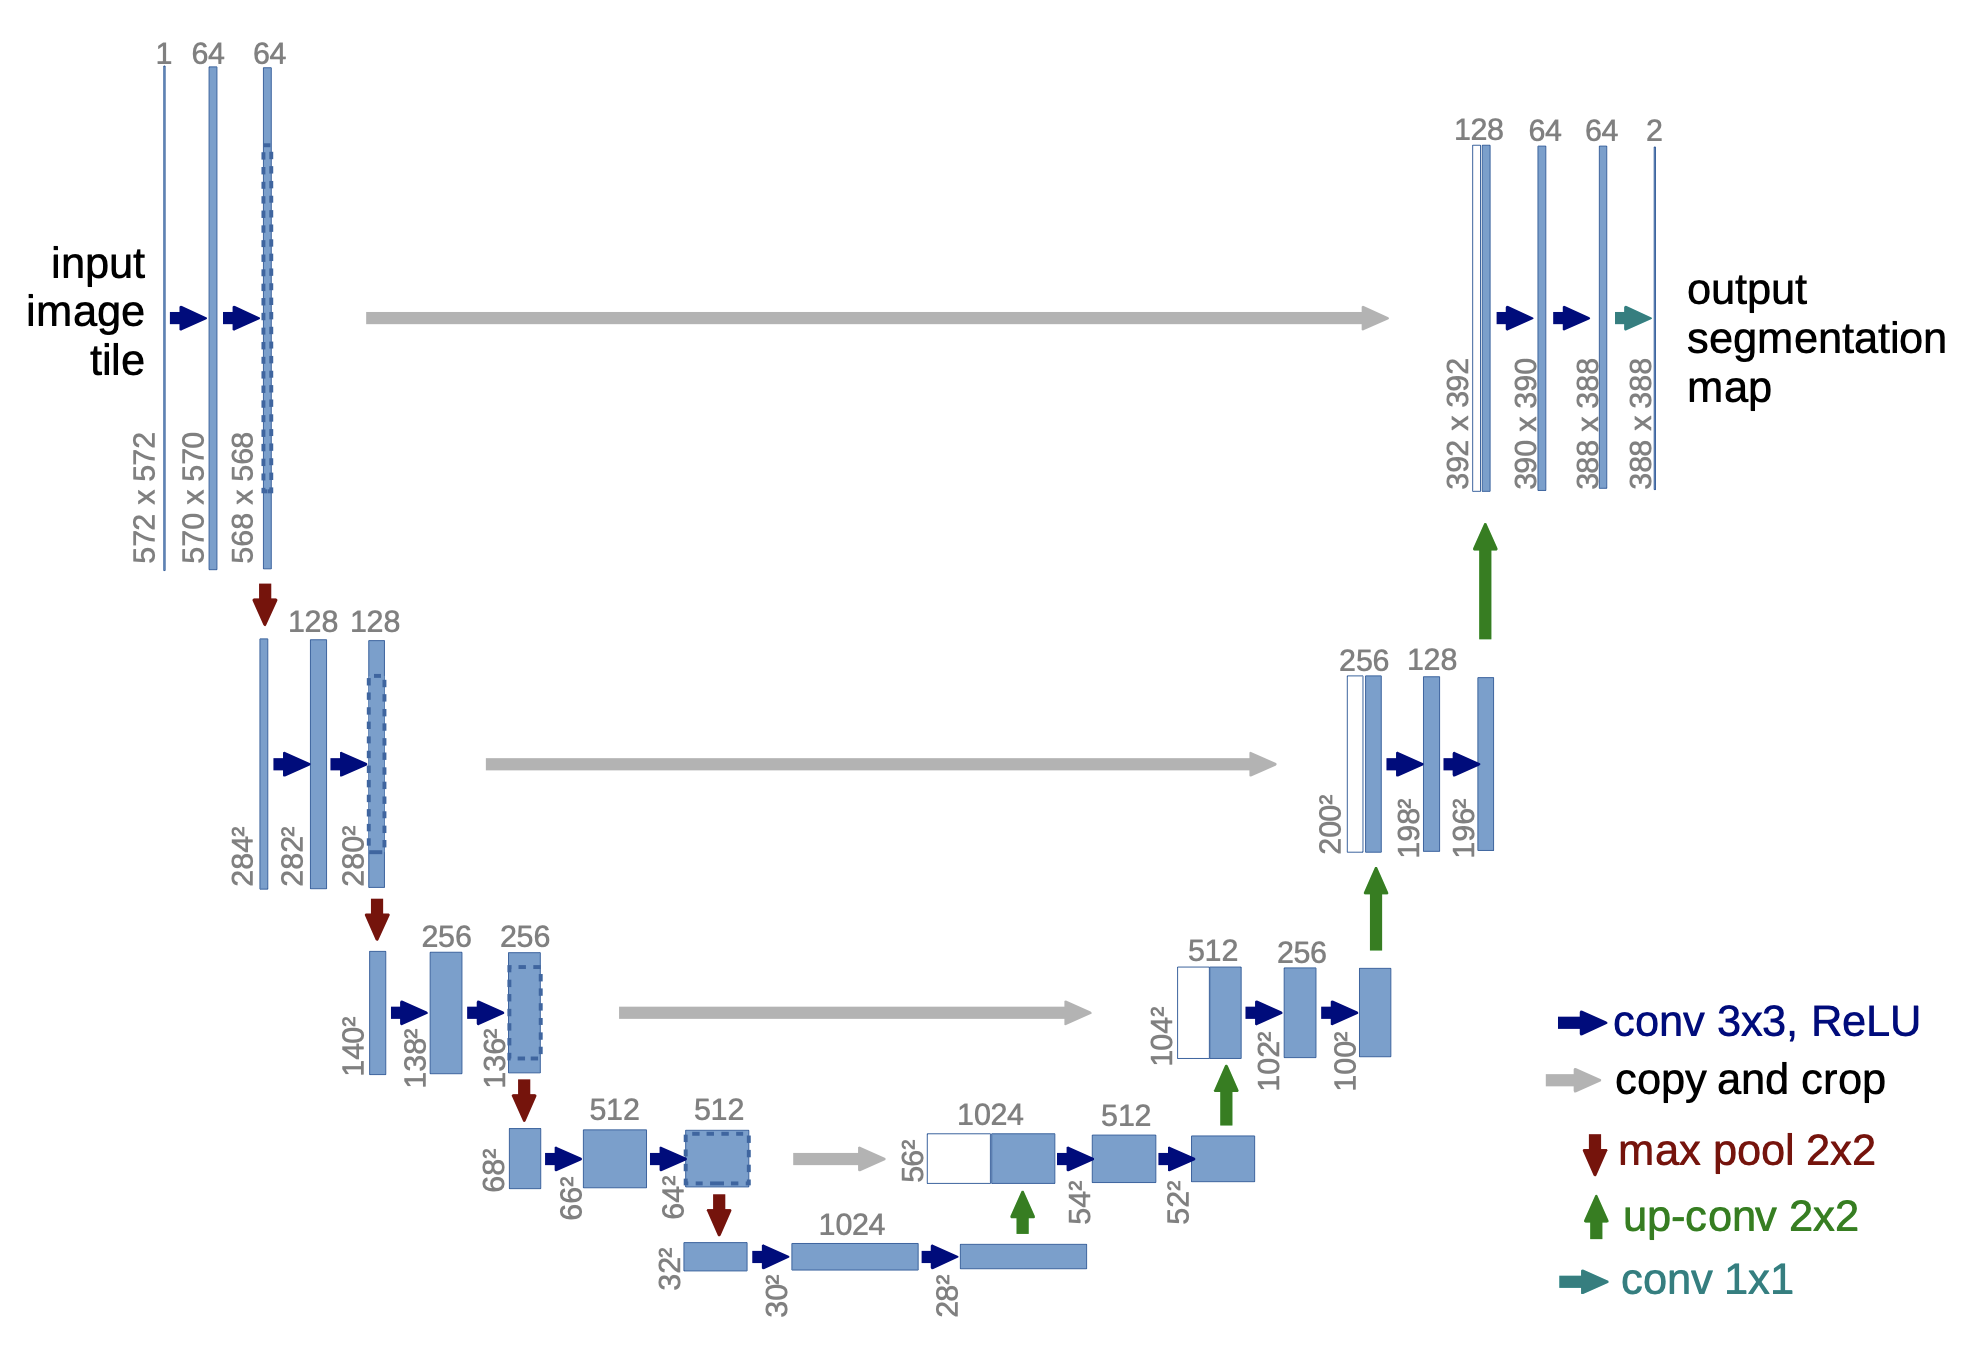
\includegraphics[scale=0.42]{img/Chap1/UNET.png}
		\caption{U-Net architecture example. Each blue box corresponds to a multi-channel feature map. White boxes represent copied feature maps. The arrows denote the different operations \cite{ART:UNet}. }
		\label{fig:UNet}
\end{figure}


\subsubsection{Atlas based Segmentation}

Another technique consists in have a sort of template already segmented (the atlas) and registering it on the image that is intended to be segmentated. This could lead to a transfer of the labels found on the atlas to the image \cite{ART:Withey}.

An atlas is a segment image of a composite head image formed from co-registered head images of several subjects \cite{ART:Withey}.
In an atlas the pixel intensity could be the simple average of the pixel intensity of the co-registered images, or it can be normalized in some arbitrary way \cite{MNI152_06}.
Another useful atlas can be tissue-type atlas, in which pixel value represents the probability of that pixel to belong to a determined tissue \cite{ART:SPAM}.

This technique consists in finding the right registration for the atlas that have to be already segmented for the classes searched. Once the atlas is registered is possible to apply the same transformation to the labels done on the atlas, in this way the labels will be transformed in the image space. 
As for the other techniques this one can be used standalone but have a great potentiality when pipelined with some others.
 
For example it is possible to register a probabilistic atlas over an unsegmented volume and using that to select the "a priori" probability for the statistical pattern recognition segmentation, as done in this work of thesis.

Finally it must be mentioned the use of probabilistic atlas had lead to the full segmentation of brain, including subcortical structures \cite{ART:Withey}.



\section{Performance Evaluation Metrics}
Once a pipeline of segmentation is implemented it is recommended to evaluate its performance. In order to do that evaluation in this work of thesis a series of methods and metrics are used. In first place to compute a metric there is the need for understanding what is a \emph{confusion matrix}. Next the main metrics for the classification are reported, such as \emph{precision, recall, specificity} and \emph{FPR}. Then more specific metrics such as \emph{accuracy, dice coefficient, jaccard index, mcc} and \emph{ROC AUC} are discussed.

\paragraph{Confusion Matrix}
As a first thing it is necessary to define the four cases that is possible to encounter during a binary classification:
\begin{itemize}
\label{Def:confusion_matrix}
    \item \texttt{True Positive (tp)}: an element that has been classified as positive while really being positive;
    \item \texttt{True Negative (tn)}: an element that has been classified as negative while really being negative;
    \item \texttt{False Positive (fp)}: an element that has been misclassified as positive while in reality is negative;
    \item \texttt{False Negative (fn)}: an element that has been misclassified as negative while in reality is positive.
\end{itemize} 

Given those definitions is possible to define the confusion matrix, that is a table that permits the visualization of the performance of classifier. Each row of the matrix represents the instances in an actual class (i.e. the \emph{ground truth}) while each column represents the instances in a predicted class. (In literature is also possible found the opposite, both variant are permitted \cite{ART:ConfusionMatrix1, ART:ConfusionMatrix2} )

\begin{figure}[h!]
		\centering
             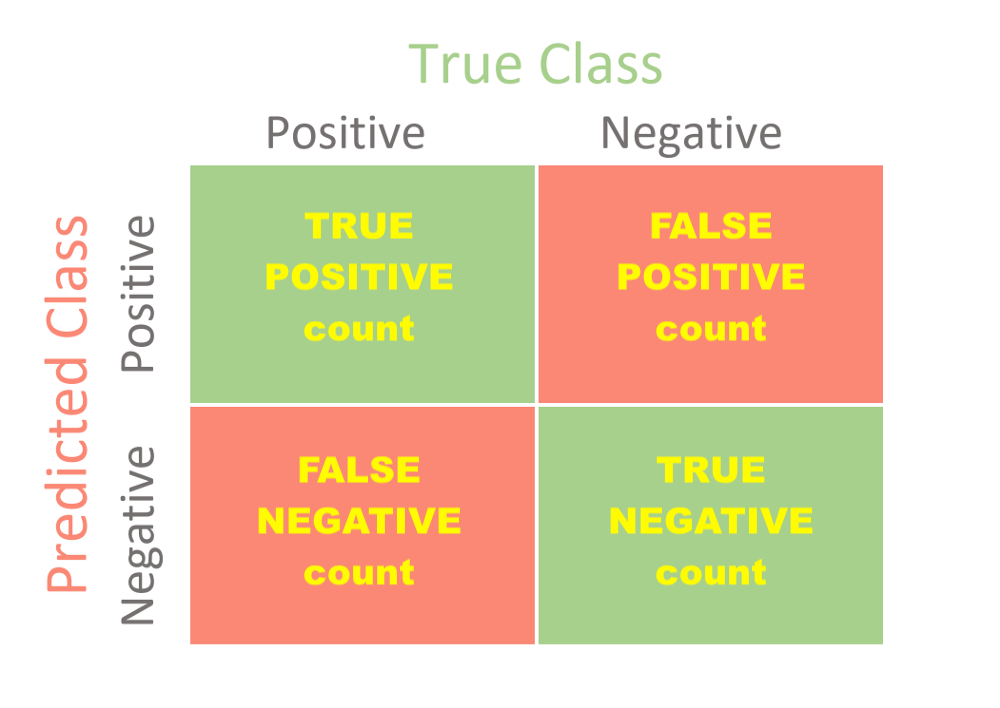
\includegraphics[scale=0.3]{img/Chap1/Confusion Matrix.png}
		\caption{Example of a binary confusion matrix. In this matrix we can find displaced all the outcomes of the classification used. In the rows are visualized the predicted classes and in the columns the actual classes of the incoming data. That permits to have a visual indication of the performance of a classificiation algorithm.  }
		\label{fig:ConfusionMatrix}
\end{figure}


\paragraph{Precision}
is the rate between the true positives and the number of all the elements predicted as positive. Intuitively is the ability to don't misclassify a negative element as positive. In the subsequent Equation \ref{eq:precision} there is the mathematic definition:
\begin{equation} \label{eq:precision}
    precision = \frac{tp}{tp+fp}
\end{equation} 


\paragraph{Recall}
, also known as \textit{true positive rate (TPR)} or \textit{sensitivity} is the rate between the true positives and all the elements that really are positive (Equation \ref{eq:recall}). It can be considered as the ability to correctly classify a positive element.
\begin{equation} \label{eq:recall}
    recall = \frac{tp}{tp+fn}
\end{equation} 

\paragraph{Specificity}
is the rate between the true negatives and all the elements that really are negative (Equation \ref{eq:specificity}). It can be considered as the ability to correctly classify a negative element.
\begin{equation} \label{eq:specificity}
    specificity = \frac{tn}{tn+fp}
\end{equation} 



\paragraph{False Positive Rate (FPR)}
is the rate between false positives and the total negatives. As visible in Equation \ref{eq:fpr} the total number of real negatives is the sum the true negatives and the false positives.
\begin{equation} \label{eq:fpr}
    FPR = \frac{fp}{tn+fp}
\end{equation} 


\paragraph{Accuracy and Balanced Accuracy}
The accuracy is the rate between the number of well estimated (true) outcomes with respects to the total outcomes (Equation \ref{eq:accuracy}) and it intuitively represents the fraction of well classificated elements with respect to the total number:
\begin{equation}
\label{eq:accuracy}
    accuracy = \frac{tp + tn}{tp + tn + fp + fn}
\end{equation}

When the two classes (positive and negative) are not composed of roughly the same amount of data, usually referred as a situation of \textit{unbalanced data}, the accuracy is not a good measure of the goodnes of a classification, due to the low reppresentation of a class in the total amount of the data.

To overcome this issue another metric was defined with the name of balanced accuracy, which is the mean of recall and specificity (Equation \ref{eq:balanced_accuracy}).
\begin{equation}\label{eq:balanced_accuracy}
    \text{balanced accuracy} = \frac{1}{2} \left( \frac{tp}{tp+fn} + \frac{tn}{tn+fp} \right) 
\end{equation}


\paragraph{Dice Similarity Coefficient / F1 score}

is used to measure the similarity of two samples. In the case of two images the similarity can be thought as the capability of the two images to overlay one on the other.
It is the double of the rate between the cardinality (number of elements in the set) of the intersection between two sets and the sum of the cardinalities of the single sets (Equation \ref{eq:Dice}). It is intuitively that the best value is $1$ (total overlapping) and the worst value is $0$ (no overlapping).
Given two sets named $X$ and $Y$ the following is the mathematical definition:

\begin{equation} \label{eq:Dice}
    DSC = 2\frac{|X \cap Y |}{|X| + |Y|}
\end{equation}

When applied to boolean data it is often referred as \textit{F1 score} and is defined as the harmonic mean of precision and recall (Equation \ref{eq:F1}).
\begin{equation} \label{eq:F1}
    F1 =\frac{2}{precision^{-1} + recall^{-1}} 
    = 2 \times \frac{precision \times recall}{precision + recall} 
    = \frac{2tp}{2tp + fp + fn}
\end{equation} 

While not immediately obvious at a first sight, the proof of the equality of those equations is reported in Appendix \ref{APPENDIX:Dice_F1}.


\paragraph{Jaccard index}
, also known as Jaccard similarity coefficient, is a metric used to evaluate overlapping between two sets. It is defined as the rate between the cardinality of intersection of the sets and the cardinality of the union of the same sets (Equation \ref{eq:Jaccard}). Given $X$ and $Y$ as the sets to evaluate:
\begin{equation}\label{eq:Jaccard}
    J = \frac{|X \cap Y|}{|X \cup Y|}
\end{equation}

\paragraph{Matthews correlation coefficient (MCC)}
, so called because was firstly used by Matthews in 1975 \cite{ART:Matthews}, is a value that ranges between $-1$ and $+1$ and can be applied to multiclass classification. Here it is discussed and defined (Equation \ref{eq:MCC}) only the case of binary classification.
The $+1$ result means a total agreement while a $-1$ means total disagreement. If the result is $0$ than the prediction is totally random \cite{ART:Baldi}.
\begin{equation}\label{eq:MCC}
    MCC = \frac {tp \times tn - fp \times fn}
                {\sqrt{(tp + fp)(tp + fn)(tn + fp)(tn + fn)}}
\end{equation}

\paragraph{Receiver Operating Characteristic (ROC) curve}
Considering a soft segmentation output in which the output is continue, to determine the classification (hard segmentation) it is necessary to apply a threshold to the outcomes of the segmentation and tp, tn, fp and fn will vary with the threshold. Usually there is a trade off between fp and fn produced by the algorithm.
ROC curve visualize this result plotting the recall in function of the false positive rate while varying the threshold \cite{ART:Baldi}.

We can distinguish two extreme curves:
\begin{enumerate}
    \item a line with $45°$ of inclination, representing a random classifier with no benefit;
    \item a broken line rising from the origin of axis to the point (0,1) and then ending at (1,1) meaning a perfect classifier.
\end{enumerate}

\paragraph{Precision-Recall Curve}

Similarly to the ROC curve, the precision-recall curve plot the trade off between the precision and the recall at the variation of the decision threshold.
This curve returns a better visualization for the goodness of a classification when the data are unbalanced, i.e. one of the two classes is less represented in the considered sample than the other \cite{ART:AUCPR}.

While the perfect classifier is represented by an horizontal line starting from the point $(1,1)$, reaching the point $(1,1)$ and then falling to the point $(1,0)$, a random classifier is represented by an horizontal line at the height equal to the rate between the positive and negative class.


\end{document}